\usetikzlibrary{calc}
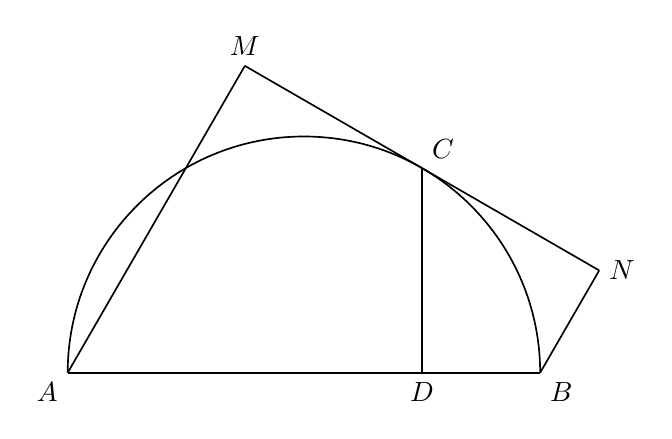
\begin{tikzpicture}[x=1cm,y=1cm,line width=.6pt,font=\normalsize]
\coordinate (O) at (0,0);
\coordinate (A) at (-3,0);
\coordinate (B) at (3,0);
\coordinate (C) at (1.5,2.598076211353316);
\coordinate (D) at (1.5,0);
\coordinate (M) at (-0.75,3.897114317029974);
\coordinate (N) at (3.75,1.299038105676658);
\draw (A) arc[start angle=180,end angle=0,radius=3cm];
\draw (A)--(B);
\draw (A)--(M);
\draw (M)--(N);
\draw (N)--(B);
\draw (C)--(D);
\node[below left] at (A) {$A$};
\node[below right] at (B) {$B$};
\node[above right] at (C) {$C$};
\node[below] at (D) {$D$};
\node[above] at (M) {$M$};
\node[right] at (N) {$N$};
\end{tikzpicture}
